\documentclass[12pt]{article}

\usepackage{amsmath}
\usepackage{latexsym}
\usepackage{amstext}
\usepackage{array}
\usepackage{multirow}
\usepackage{graphicx}
\usepackage{caption}
\usepackage{subcaption}


%\usepackage{subcaption}

\pagestyle{plain}


\begin{document}
\title{Random loops -Supplementary material}

\begin{figure}[H]
 \begin{subfigure}[b]{0.3\textwidth}
 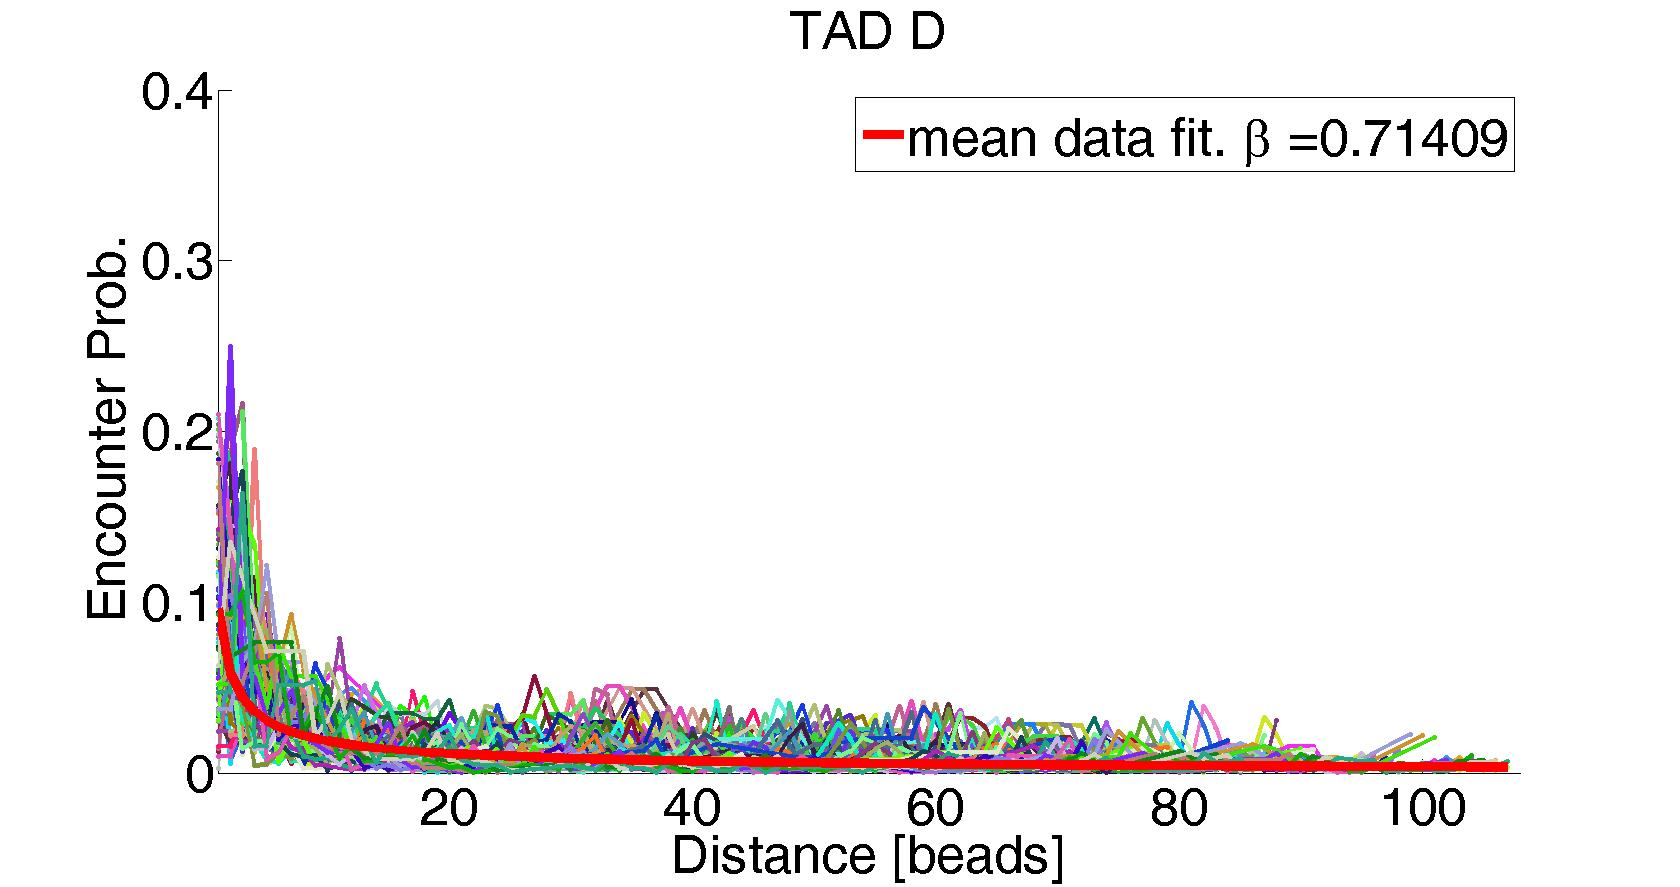
\includegraphics[scale=0.2]{meanDataFitTADD}
 \caption{}
 \end{subfigure}
 
 \begin{subfigure}[b]{0.3\textwidth}
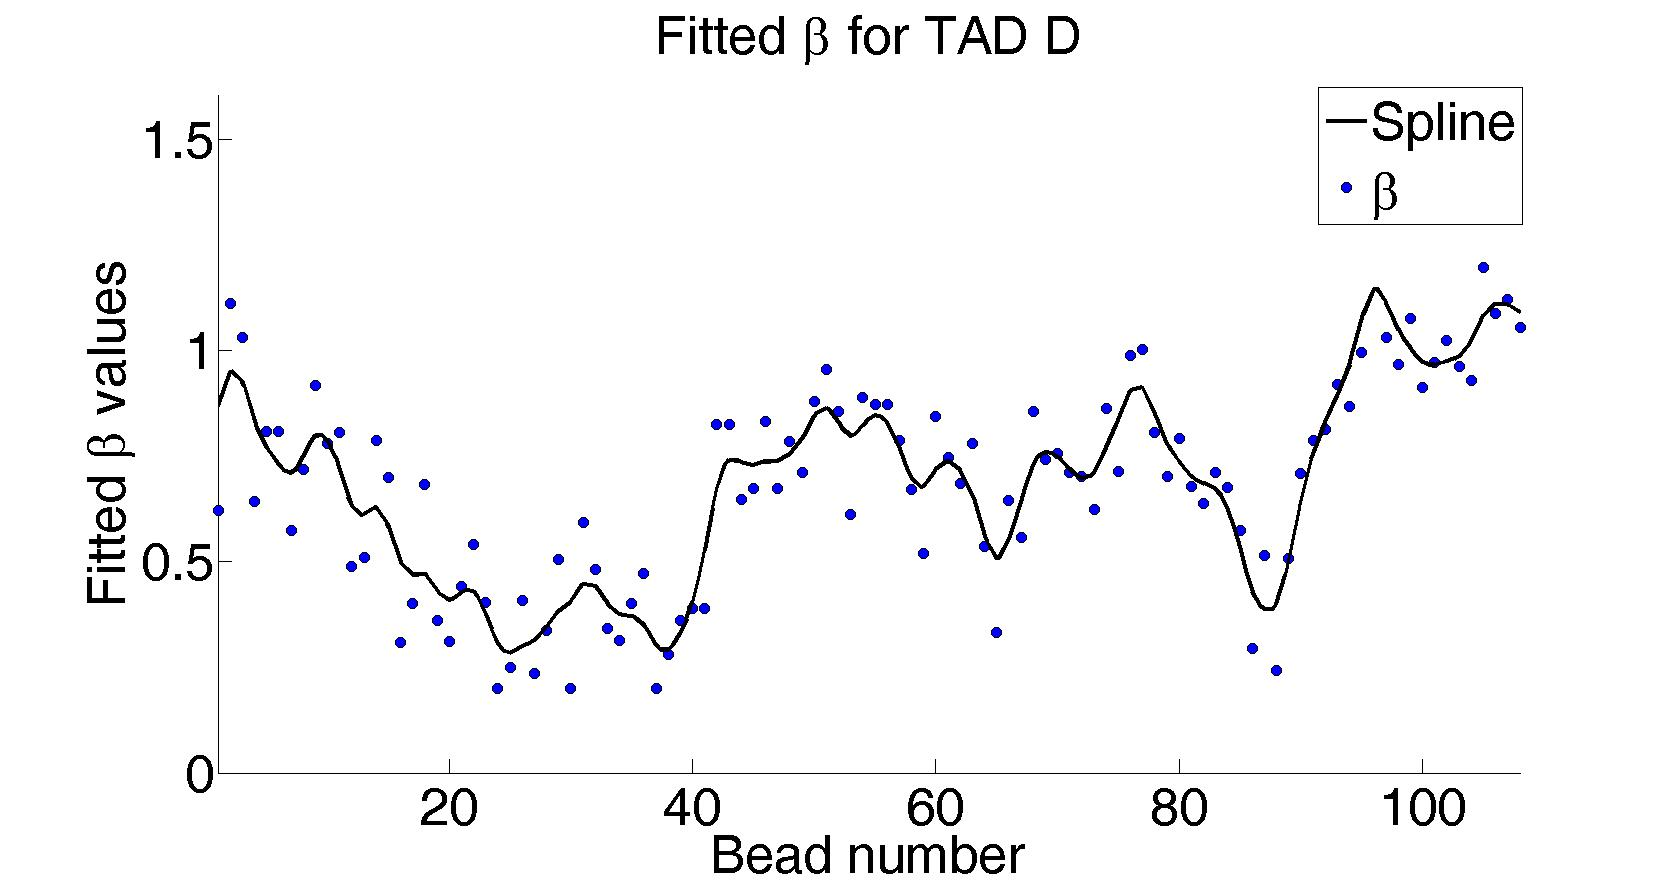
\includegraphics[scale=0.2]{fittedExpValuesWithSplineAverageTADD}
\caption{}
 \end{subfigure}
\caption{The encounter probability and the fitted $\beta$ values for TAD D.}
\end{figure}

\begin{figure}[H]
 \begin{subfigure}[b]{0.3\textwidth}
 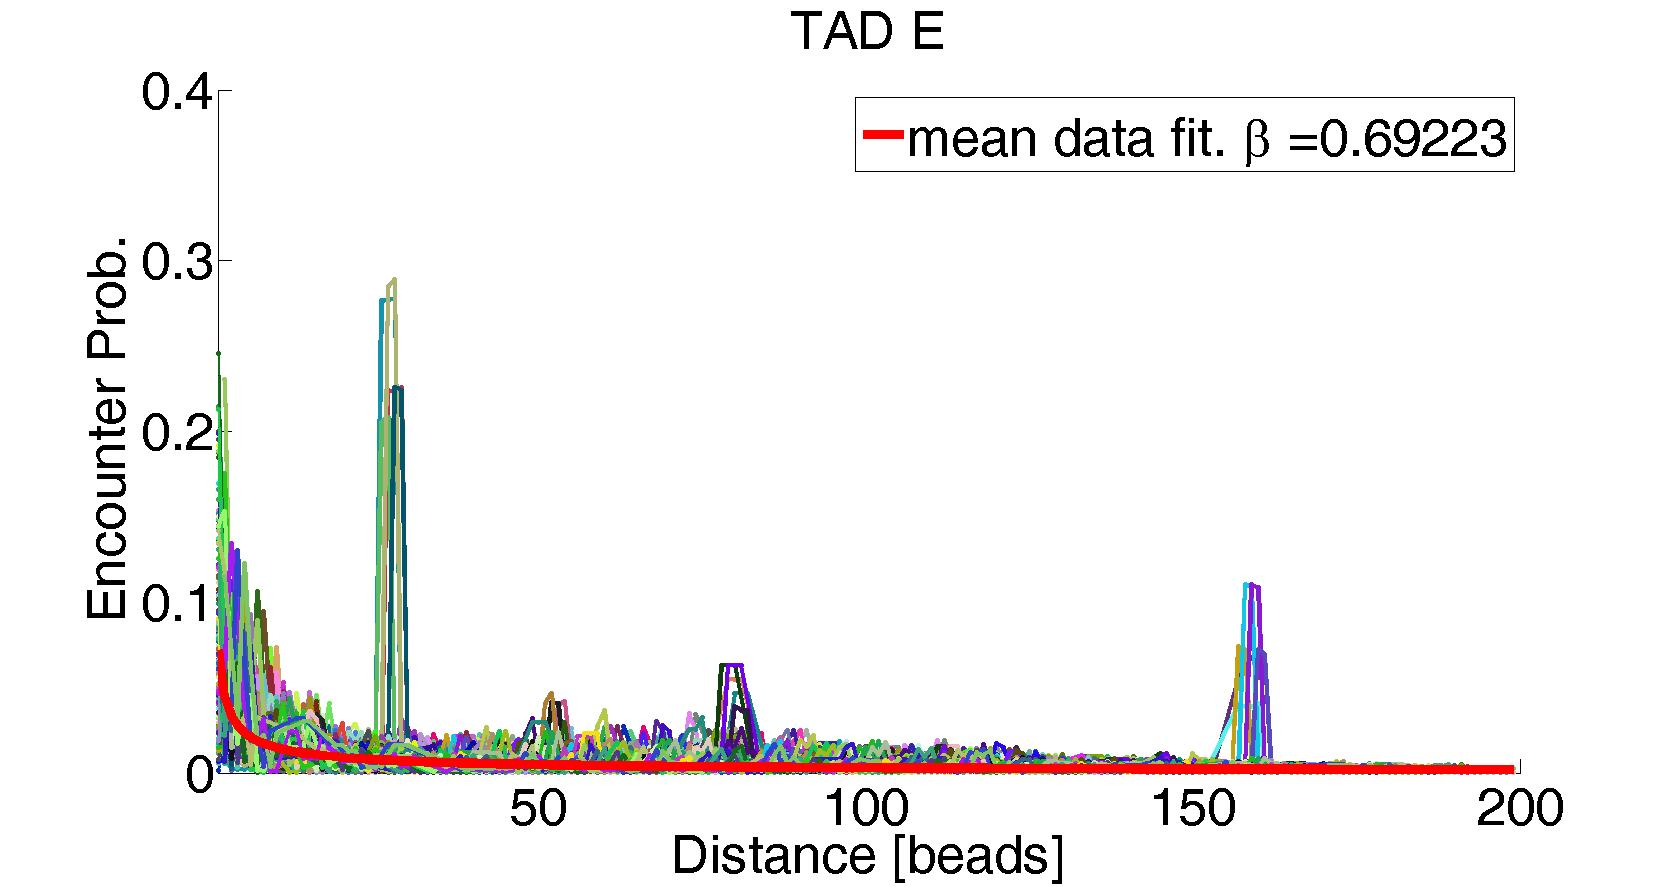
\includegraphics[scale=0.2]{meanDataFitTADE}
 \caption{}
 \end{subfigure}
 
 \begin{subfigure}[b]{0.3\textwidth}
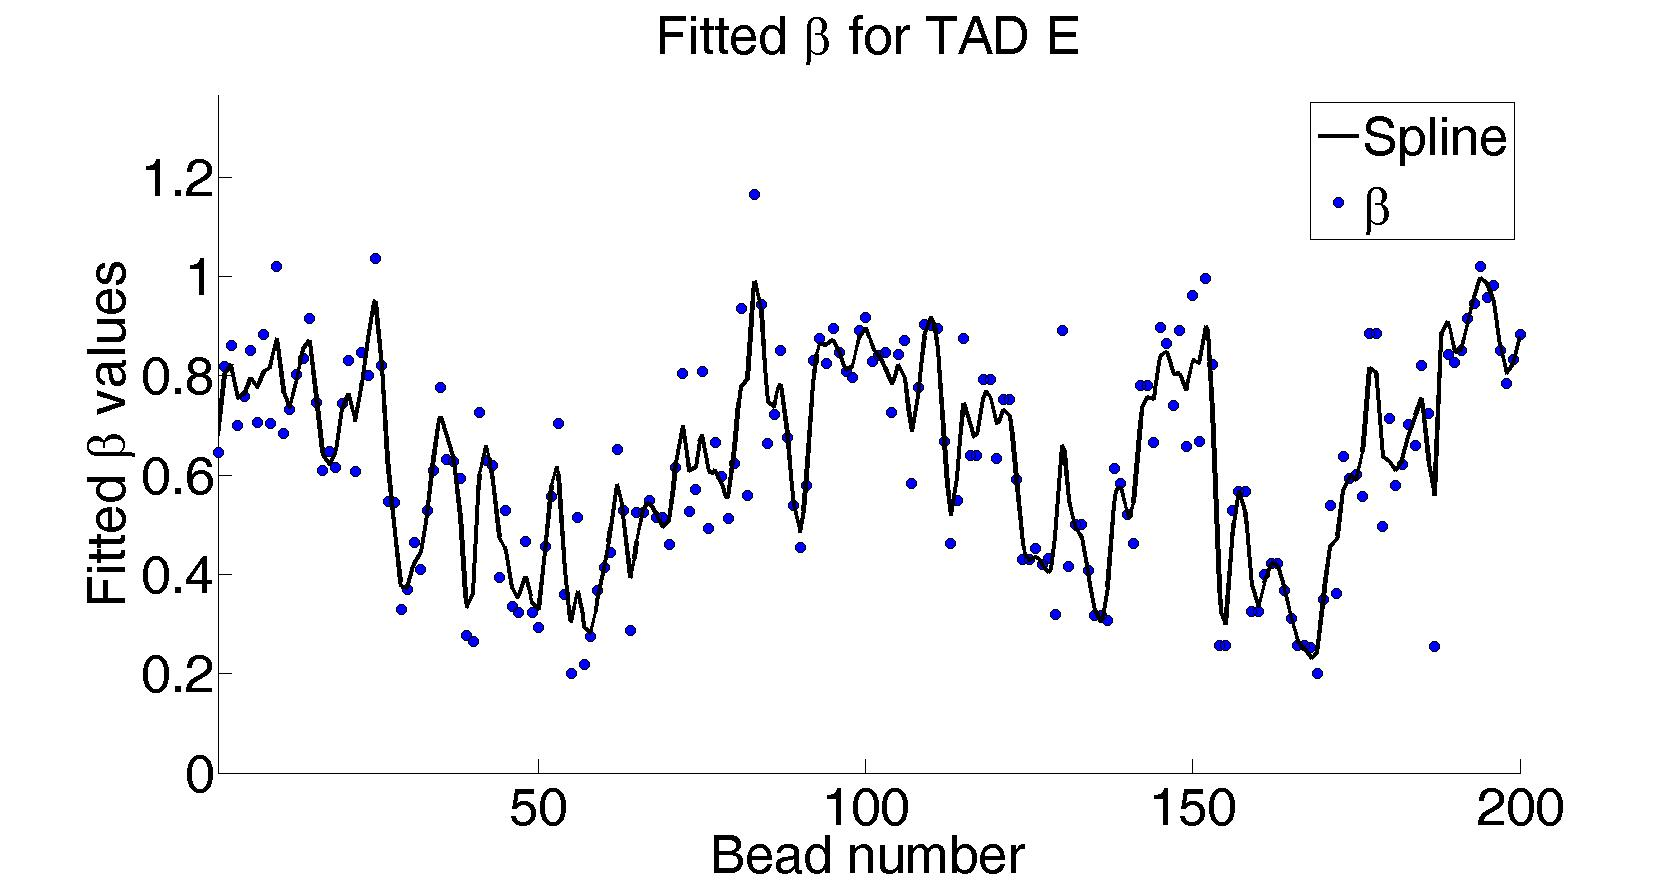
\includegraphics[scale=0.2]{fittedExpValuesWithSplineAverageTADE}
\caption{}
 \end{subfigure}
\caption{The encounter probability and the fitted $\beta$ values for TAD E.}
\end{figure}
\subsection{Peak Calling}
To accurately identify pair of beads that interact more frequently than expected, we ran a peak calling procedure on the 5C probability data of each TAD separately. For each bead $i=1..N$ of the chain, we fit an encounter probability curve of the form 
$\alpha_i d^{-\beta_i}$. We then use the values of the fitted curves at each distance $d=1..(N-1)$  to estimate the expected encounter probability, $\mu(d) = E[\alpha_i d^{-\beta_i}]$, and the expected standard-deviation, $\sigma(d)=\sqrt{E[(\mu(d)-\alpha_i d^{-\beta_i})^2]}$, for each $d$, and $i=1...N$. 

For each observation $i$ at distance $d$ we calculate a z-score by $z_i(d)=\frac{|\alpha_i d^{-\beta_i}-\mu(d)|}{\sigma(d)}$ and fit a Weibull distribution to it. For each z-score a p-value is calculated based on the fitted Weibull CDF and then transformed into a q-value to obtain false discovery rate. We then threshold the data using false discovery rate of 0.01.

The automated procedure resulted in 62 peaks in TAD E, and 




\end{document}